\documentclass[reprint,pra, twocolumn, amsmath,amssymb,
 aps,superscriptaddress,]{revtex4-2}

\usepackage[utf8]{inputenc}
\usepackage[english]{babel}
\usepackage[a4paper,margin=2.0cm]{geometry}

\makeatletter
\setlength{\@fptop}{0pt}
\makeatother

\columnsep=1.0pc
\parindent=1.0cm
\parskip=6.0pt
\usepackage{amsmath,amsfonts,amssymb,dsfont,amsthm}
\usepackage{indentfirst}
\usepackage{graphicx}
\usepackage{booktabs}
\usepackage{siunitx}
\usepackage{lipsum}
\usepackage{listings}
\sisetup{output-decimal-marker={,}}
\sisetup{use-xspace}
\sisetup{space-before-unit}
\sisetup{angle-symbol-over-decimal}
\sisetup{group-digits=false}
\DeclareMathOperator{\Tr}{Tr}
\usepackage{tasks}
\usepackage{amssymb}
%\usepackage{wasysym}
\usepackage[T1]{fontenc}
%\usepackage{authblk}
%\usepackage[raggedright]{titlesec}

\usepackage{comment}
\usepackage{mathtools}
\usepackage{extpfeil}
\usepackage{xcolor}
\usepackage{hyperref}
\usepackage{url}
\usepackage{natbib}
\usepackage{makecell}

\usepackage{physics}
%\AtBeginDocument{\RenewCommandCopy\qty\SI}
\usepackage{graphicx}% Include figure files
\usepackage{dcolumn}% Align table columns on decimal point
\usepackage{bm}% bold math
\usepackage{tikz}
\usepackage{pgf}
\usepackage{tikzscale}
\usetikzlibrary{angles,calc,intersections,quotes,arrows.meta, shapes,decorations.markings, external}
%\tikzexternalize


\newtheorem{thm}{Theorem}%[section]
\newtheorem{lem}{Lemma}
\newtheorem{prop}{Proposition}
\newtheorem{cor}{Corollary}
\newtheorem{defi}{Definition}
\newtheorem{rem}{Remark}
\newtheorem{ex}{Exercise}
\newtheorem{eg}{Example}
\newtheorem{obs}{Observation}

\newcommand{\ie}{\textit{i.e.}}
\newcommand{\eq}{Eq.}
\newcommand{\muns}{$\mu^{\text{NS}}$}
\newcommand{\alice}{$\mathcal{A}$}
\newcommand{\bob}{$\mathcal{B}$}

\newcommand{\noob}[1]{\textcolor{blue}{[A:#1]}}
\newcommand{\lu}[1]{\textcolor{red}{[L:#1]}}

\newcommand{\ba}[1]{\begin{align} #1 \end{align}}
\newcommand{\bfr}[2]{\begin{frame}{#1} #2 \end{frame}}
\newcommand{\bi}[1]{\begin{itemize} #1 \end{itemize}}
\newcommand{\be}[1]{\begin{enumerate} #1 \end{enumerate}}
\newcommand{\beq}[1]{\begin{equation} #1 \end{equation}}
\newtheorem{lemma}{Lemma}
\newtheorem{result}{Result}




\date{January 2026}

\begin{document}



\title{The entropic approach for quantum networks: Notes}

\author{}
\email{}
\affiliation{}

\begin{abstract}

%Abstract: Here we address the problem of certifying nonclassicality in Bell scenarios with independent sources. Such independence constraints make the problem non-convex, significantly increasing the computational complexity. The inflation technique provides a tool to enhance nonclassicality certification by mapping the problem to more stringent scenarios. However, the problem remains non-convex, and the methods can only be applied in scenarios with small cardinalities. Here, we introduce the entropic framework to efficiently tackle this computational complexity. In this approach, the use of entropies makes the independence relations linear constraints, keeping the problem convex. We show that the entropic framework can witness nonclassicality in the most common scenarios and derive entropic witnesses well known in the current literature. Moreover, we investigate the performance of the entropic method in scenarios where current methods are intractable in practice.
    
\end{abstract}
\maketitle
\onecolumngrid

\section{The entropic approach}
In Bell scenarios with independent sources, we typically consider a network of observed variables and unobserved systems connected to these variables. One way to analyze these networks is to use entropy vectors $H$, i.e., vectors whose components correspond to the entropies of each subset of observed variables. The starting point for deriving entropic constraints within causal structures is the so-called \emph{Shannon inequalities}
\begin{align*}
    &H(X)\geq 0 \\
    &H(X|Y):= H(X,Y)-H(Y)\geq 0\\
    &I(X:Y|Z):=H(X,Z)+H(Y,Z)-H(Z)-H(X,Y,Z)\geq 0
\end{align*}
which are non-negativity of entropy, conditional entropy and conditional mutual information and where $X$, $Y$, $Z$ are sets of disjoint variables. They are known to constrain a convex polyhedral cone, the \emph{Shannon cone}. In fact, we can equivalently describe the Shannon cone with the set of minimal \emph{elemental inequalities}. If we consider $n$ random variables, $X_1$, ..., $X_n$,  given by 
\begin{align*}
    &H(X_i|\{X_1,..., X_n/X_i\})\geq 0\quad \forall i\\
    &I(X_i,X_j|\{X_1,..., X_n/X_i,X_j\})\geq 0\quad \forall i\neq j
\end{align*}
and the number of elemental inequalities is $n+\binom{n}{2}2^{n-2}$. Then, we impose the conditional independences of the variables in the network. These are given by 
\begin{equation}
    I(X_i: \text{ND}(X_i)|\text{Pa}(X_i))=0\quad \forall i,
\end{equation}
where ND$(X_i)$ are the \emph{non-descendants} of $X_i$, and Pa$(X_i)$ are the \emph{parents} of $X_i$. By imposing these conditions, we constrain the Shannon cone to the set of entropy vectors which are compatible with a given causal structure. 

For simplicity, let us consider the paradigmatic example of the triangle network, where we have the observed variables $A$,$B$,$C$ and the unobserved variables $\alpha$, $\beta$ and $\gamma$ that connect $BC$, $AC$ and $AB$ respectively. Here, in addition to the elemental inequalities of $H(A,B,C,\alpha,\beta,\gamma)$, we have 
\begin{align*}
    &I(A : B,C ,\alpha \mid \beta,\gamma)=0\\
    &I(B : A,C ,\beta \mid \alpha,\gamma)=0\\
    &I(C : A, B, \gamma \mid \beta, \alpha)=0
\end{align*}
in entropic terms, and the independence of the unobserved variables is fully captured by $H(\alpha, \beta, \gamma) = H(\alpha) + H(\beta) + H(\gamma)$. In general, these conditions can be formulated as a Linear Program
\begin{align}\label{lp:feas_E}
     \underset{\mathbf{H}}{\text{minimize}} &\quad  0 \nonumber\\
    \text{subject to}&\quad E\cdot\mathbf{H}\ge \vec{0}\nonumber\\
    &\quad R\cdot\mathbf{H} =  \vec{0}\nonumber\\
\end{align}
where $\mathbf{H}$ is the entropic vector, $E\cdot\mathbf{H}\ge \vec{0}$ represents the elemental inequalities, and $R\cdot\mathbf{H} =  \vec{0}$ represents the variables' independences in the network. This approach can already yield some non-trivial conditions, i.e. we can consider the projection of the conditions in \ref{lp:feas_E} over the observed variables $\{ H(A),H(B),H(C),H(A,B), H(A,C), H(B,C), H(A,B,C) \}$.
\textcolor{red}{[Test all inequalities.]}

%Consider a probability distribution of observable variables of interest $\mathbf{p}_{\text{NC}} = \{p(a,b,...,c)\}$. The nonclassicality certification problem consists of checking the feasibility of the problem:
%
%\begin{align}\label{lp:feas}
  %  \underset{\mathbf{P}}{\text{minimize}} &\quad  0 \nonumber\\
  %  \text{subject to}&\quad M_C\cdot\mathbf{P}\le \vec{b}\\
  %  &\quad P(\alpha_1 , \alpha_2, ..., \alpha_n) =\prod_i^n P(\alpha_i) \nonumber\\
   % & \quad \mathbf{p} = \mathbf{p}_{\text{NC}}\nonumber
%\end{align}
%
%where $\mathbf{P}$ denotes the full joint probability distribution, including all observed and latent variables, from which the distribution of observable variables $\mathbf{p}$ can be obtained via marginalization $p(a,b,...,c) = \sum_{\{\alpha_i\}_i} p(a,b,...,c, \alpha_1, ...\alpha_n)$. The matrix $M_C$ encodes all the linear constraints implied by the causal structure. $P(\alpha_1 , \alpha_2, ..., \alpha_n)$ denotes the probability distributions related to the sources $\alpha_i$, which are independent of each other. If problem \eqref{lp:feas} is infeasible, $\mathbf{p}_{\text{NC}}$ is nonclassical.

%Equivalently, we can describe the problem in terms of entropies. In this case, the distribution $\mathbf{p}_{\text{NC}}$ implies some of the components of the entropic vector $\mathbf{H}$, whose components are given by the joint entropies of all possible combinations of variables of the problem, where:
%
%\begin{align}
%    H(X_1,...,X_n) = -\sum p(x_1, ... x_n)\log_2\left[p(x_1, ... x_n)\right]. \nonumber
%\end{align}
%
%In this case, the problem \eqref{lp:feas} can be equivalently written as:
%
%\begin{align}\label{lp:feas_E}
   % \underset{\mathbf{H}}{\text{minimize}} &\quad  0 %\nonumber\\
   % \text{subject to}&\quad B_C\cdot\mathbf{H}\ge \vec{0}\\
   % &\quad E_C\cdot\mathbf{H} =  \vec{0}\\
   % &\quad H(\alpha_1 , \alpha_2, ..., \alpha_n) =\sum_i^n %H(\alpha_i) \nonumber\\
  %  & \quad \mathbf{h} = \mathbf{h}_{\text{NC}}\nonumber
%\end{align}
%
%where $B_C$ encodes all basic inequalities constraining the entropic vector, and $E_C$ encodes all causal relations of the DAG, in terms of conditional independence relations $I(A:B|C)=0$. $\mathbf{H}$ denotes the entropic vector including all observable and latent variables. $\mathbf{h}$ denotes all components of $\mathbf{H}$ containing observable variables, and $\mathbf{h}_{\text{NC}}$ denotes all values for the components including observable variables implied by the distribution $\mathbf{p}_{\text{NC}}$. All components of $\mathbf{H}$ including sources are kept as variables. If problem \eqref{lp:feas_E} is infeasible, $\mathbf{p}_{\text{NC}}$ is nonclassical.

%Notice that the feasibility problem provides a sufficient criterion to identify nonclassicality, but if the problem is found feasible, we cannot conclude that the distribution is classical. The inflation technique states that the nonclassicality of a distribution associated with a certain causal structure may be witnessed in a larger causal structure containing the original DAG. In fact, the inflation technique consists of finding these suitable larger DAGs enabling the witnessing of such nonclassicality. In this case, the entropic vector $\mathbf{H}$ includes these extra components associated with the additional variables from the inflated DAG, and the problem requires including consistency constraints related to the inflation technique. 

\begin{figure}[t]
    \centering
    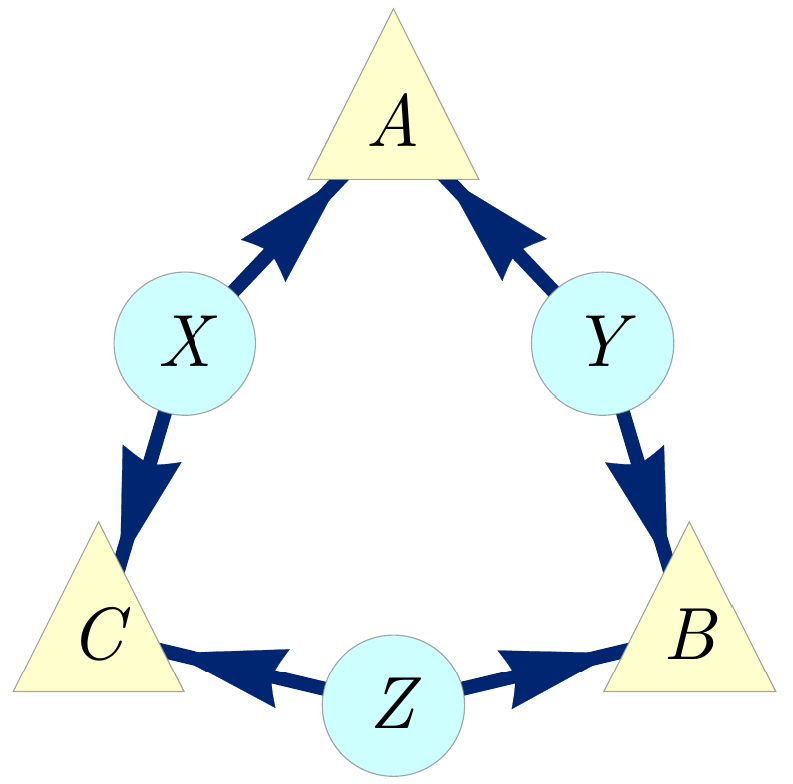
\includegraphics[width=0.3\linewidth]{triangle.png}\quad\quad\quad
    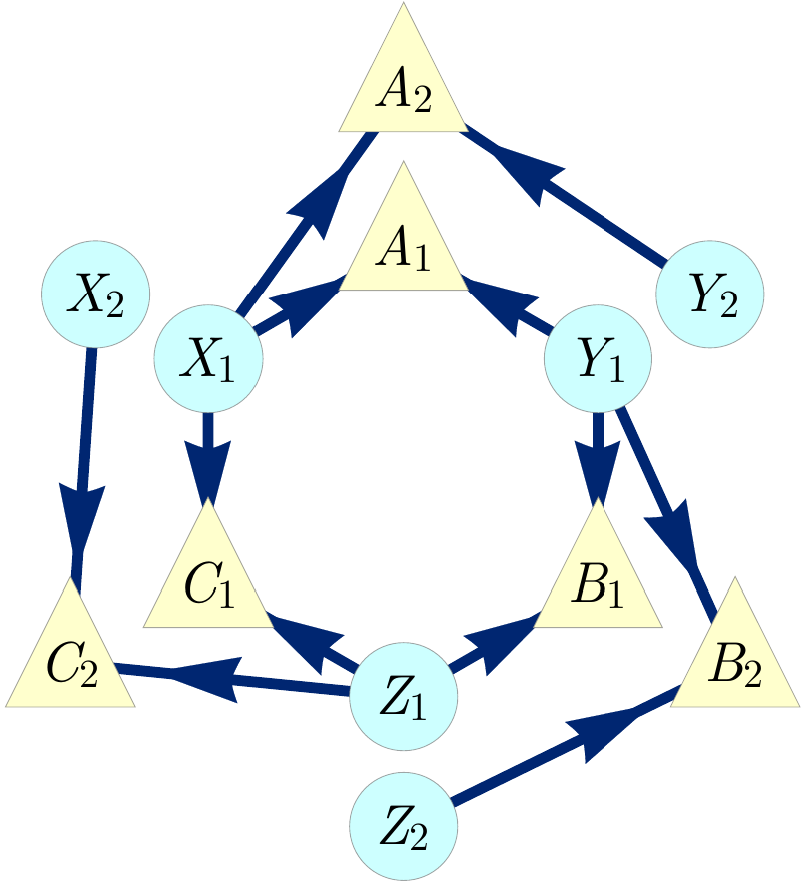
\includegraphics[width=0.3\linewidth]{spiral.png}\\Triangle \quad\quad \quad Spiral
    \caption{Triangle and Spiral inflation}
    \label{fig:triangle}
\end{figure}


\subsection{Triangle}

Before proceeding to describe the inflated scenarios, it is important to obtain the information-theoretic description of the standard triangle scenario. In this case, we consider the set of variables given by $S = \{A_0, B_0, C_0, \alpha_0, \beta_0, \gamma_0\}$. Since we are describing the complete set of variables, the causal relations are fully captured by Pearl's criterion: a probability distribution $P$ is compatible with a causal structure if and only if every variable in the DAG is independent of its non-descendants, conditioned on its parents. That is, given a DAG with variables $\{X_i\}_{i=0}^{n-1}$, we have $X_i \perp \{Y / X_i, PA_i\} \mid PA_i$ for all $i$, where $PA_i$ denotes the set of parent variables of $X_i$. In this case, the variables form a Bayesian network, and the joint probability distribution factorizes as
\begin{align}\label{eq:Markov}
p(x_0,\ldots,x_{n-1}) = \prod_{i=0}^{n-1} p(x_i \mid x_{PA_i}).
\end{align}
Consequently, in entropic terms, Pearl's criterion implies $I(X_i : \{Y / X_i, PA_i\} \mid PA_i) = 0$ for all $i$. Thus, we can list the conditional independences of each variable with respect to its non-parental variables. For the triangle scenario, it is sufficient to consider the relations
$A_0 \perp B_0 C_0 \alpha_0 \mid \beta_0 \gamma_0$,
$B_0 \perp A_0 C_0 \beta_0 \mid \alpha_0 \gamma_0$, and
$C_0 \perp A_0 B_0 \gamma_0 \mid \beta_0 \alpha_0$.
Moreover, the independence of the sources is fully captured by
$H(\alpha_0, \beta_0, \gamma_0) = H(\alpha_0) + H(\beta_0) + H(\gamma_0)$.

Having collected all these constraints, we are now ready to solve the problem \eqref{lp:feas_E}. We test two nonclassical distributions, $\mathbf{P}{\text{GHZ}} = \{p(a,b,c)\mid p(0,0,0)=p(1,1,1) = 1/2\}$ and $\mathbf{P}{\text{W}} = \{p(a,b,c)\mid p(0,0,1)=p(0,1,0)=p(1,0,0) = 1/3\}$. The nonclassicality of $\mathbf{P}{\text{GHZ}}$ is witnessed, whereas $\mathbf{P}{\text{W}}$ is not. The robustness of the method for the given inflation is $0.707$, while state-of-the-art inflation techniques based on probabilities yield approximately $0.5$.

\section{Spiral with no sources}


Let us consider the triangle scenario depicted in Fig.\ref{fig:triangle}, where the simplest inflated DAG is given by the spiral inflation. Here we do not include the latent variables in the description and only include the independence relations implied by them. Thus, we consider only the marginal scenario $\mathcal{M} = \{A_0, B_0, C_0, A_1, B_1, C_1\}$. In this case, the causal relations can be identified by the d-separation criterion: if the paths between two random variables contain at least one collider, these variables are independent. Consider, for instance, the DAG
\begin{align}
    A\longrightarrow B \longrightarrow C \longleftarrow D
\end{align}
In this case, $p(b,d) = p(b)p(d)$. The effect of the collider on the marginals $p(a, d)$ is
%
\begin{align}
    p(a,d) &= \sum_{bc} p(a,b,c,d) \nonumber\\
            & = \sum_{bc} p(a|b)p(c|b,d)p(b)p(d) \nonumber\\
            & = \sum_{b} p(a|b)p(b)p(d) = p(a)p(d).
\end{align}
%
This directly leads to $H(A,D) = H(A)+H(D)$. We can then list all independence relations arising from colliders for the marginal scenario $\mathcal{M}$.

Consider the variable $A_0$. The only variable or subset of variables with a collider in between $A_0$ is $C_1$. That is,
%
\begin{align}
    &A_0 \longleftarrow \gamma_0 \longrightarrow B_1 \longleftarrow \alpha_0 \longrightarrow C_1 \nonumber\\
    &A_0 \longleftarrow \gamma_0 \longrightarrow C_0 \longleftarrow \alpha_0 \longrightarrow C_1
\end{align}
%
Then, $A_0\perp C_1$. By symmetry, for $B_0$ and $C_0$ we have $B_0\perp A_1$ and $C_0\perp B_1$, and any independence relation containing $A_0, B_0, C_0$ will only involve these variables. We then find the paths blocked from $A_1,B_1$, and $C_1$:
%
\begin{align}
    &A_1 \longleftarrow \beta_0 \longrightarrow A_0 \longleftarrow \gamma_0 \longrightarrow B_0 B_1 \nonumber\\
    &A_1 \longleftarrow \beta_0 \longrightarrow A_0 \longleftarrow \gamma_0 \longrightarrow B_0  \longleftarrow \gamma_0 \longrightarrow B_1 \nonumber\\
    &A_1 \longleftarrow \beta_0 \longrightarrow C_0 \longleftarrow \alpha_0 \longrightarrow B_0  \longleftarrow \gamma_0 \longrightarrow B_1 \nonumber\\
    &A_1 \longleftarrow \beta_0 \longrightarrow C_0 \longleftarrow \alpha_0 \longrightarrow C_1 \nonumber\\
\end{align}
%
Consequently, $A_1$ is independent of any variable beyond the colliders $A_0$ and $C_0$, which gives the following independence relations: $A_1\perp B_0$, $A_1\perp B_1$, $A_1\perp B_0B_1$, $A_1\perp B_0C_1$, $A_1\perp C_1$, and $A_1\perp B_0B_1C_1$. However, the only relevant ones are $A_1\perp B_0$, $A_1\perp B_1$, $A_1\perp B_0C_1$, $A_1\perp C_1$. By symmetry, we can list the relevant independence relations for $B_1$ and $C_1$, giving the complete set:
%
\begin{align}
    A_1\perp B_0, \; A_1\perp B_1, \; A_1\perp C_1\nonumber\\
    B_1\perp C_0, \; B_1\perp C_1\\
    C_1\perp A_0.\nonumber
\end{align}
Notice that the relation $H(A_1,B_1, C_1) = H(A_1)+H(B_1)+H(C_1)$ already encodes the independences $A_1\perp B_1$, $B_1\perp C_1$, $A_1\perp C_1$, which leads to the minimal set of independence relations:
%
\begin{align}
    A_1\perp B_1 \perp C_1, \; A_1\perp B_0, \; B_1\perp C_0, \; C_1\perp A_0\nonumber
\end{align}
%

At this point, the only missing constraints are those related to consistency of the marginals. In fact, $A_1,B_1,C_1, \alpha_1,\gamma_1, \beta_1$ consist of copies of the original variables from the triangle. Consequently, the marginal components of $\mathbf{H}$ including copy variables with the same parental correlating variables should match those of the original variables. Following this concept, we have the following consistency relations for the marginals associated with the spiral inflation from Fig.\ref{fig:triangle}:
%
\begin{align}\label{eq:consistency1}
    H(A_1) = H(A_0) \nonumber \\
    H(B_1) = H(B_0) \nonumber \\
    H(C_1) = H(C_0) \\
    H(A_0, B_1) = H(A_0, B_0) \nonumber \\
    H(B_0,C_1) = H(B_0, C_0) \nonumber \\
    H(C_0,A_1) = H(C_0,A_0) \nonumber
\end{align}

Having collected all these constraints, we are now ready to solve the problem \eqref{lp:feas_E}. We tested two nonclassical distributions, $\mathbf{P}_{\text{GHZ}} = \{p(a,b,c)| p(0,0,0)=p(1,1,1) = 1/2\}$ and $\mathbf{P}_{\text{W}} = \{p(a,b,c)| p(0,0,1)=p(0,1,0) =p(1,0,0) = 1/3\}$, where the nonclassicality of $\mathbf{P}_{\text{GHZ}}$ is witnessed while $\mathbf{P}_{\text{W}}$ is not. The robustness of the method for the given inflation is $0.78$. Consequently, it becomes evident that we have to include the full description in order to outperform the triangle standard description. 

Moreover, there exist two entropic witnesses of nonclassicality for the triangle scenario, which have the form
%
\begin{align}\label{eq:entropic_witness}
    H(A)+H(B)+H(C)-H(AB)-H(AC)\le 0 \\
    H(A)+H(B)+H(C)-2H(ABC)\le 0.\nonumber
\end{align}
%
Interestingly, both are implied by the constraints in \eqref{lp:feas_E} through Farkas’ lemma. This result suggests that \eqref{eq:entropic_witness} are already captured by the entropic framework with the simplest inflation.

The spiral inflation constitutes a weak inflation; the methods can be significantly improved for more refined inflations.


\section{Full Spiral}

Now we can contrast these findings by considering the full entropic description of the spiral inflation, which involves the complete set of variables of the form $\mathcal{S}=\{A_0, B_0, C_0, A_1, B_1, C_1, \alpha_0, \alpha_1, \beta_0, \beta_1, \gamma_0, \gamma_1\}$. Since we have included the whole description, we simply need to apply Pearl's criterion. Thus, from the \eqref{eq:Markov} condition, we can, for instance, include for the spiral DAG the constraint
$A_0\perp B_0 C_0 A_1 B_1 C_1 \alpha_0 \alpha_1 \beta_1 \gamma_1 \mid \beta_0 \gamma_0$,
while the other five conditional independence constraints follow analogously. Moreover, the independence of the sources is fully captured by
$H(\alpha_0, \alpha_1, \beta_0, \beta_1, \gamma_0, \gamma_1) = H(\alpha_0)+ H(\alpha_1)+ H(\beta_0)+H(\beta_1)+H(\gamma_0)+ H(\gamma_1)$.

We also include the consistency relations, which reduce the computational complexity of the problem. In this case, the relations listed in \eqref{eq:consistency1} also hold, and we can additionally impose several others. For instance, the consistency of the sources implies
%
\begin{align}
H(\alpha_0) &= H(\alpha_1),\\
H(\gamma_0) &= H(\gamma_1),\\
H(\beta_0) &= H(\beta_1).
\end{align}
%
Moreover, we can impose further marginal consistency relations of the form
\begin{align}\label{eq:consitency2}
H(A_0, \beta_0) &= H(A_1, \beta_0),\\
H(A_0, \gamma_0) &= H(A_1, \gamma_1),\\
H(A_0, \beta_0, \gamma_0) &= H(A_1, \beta_0, \gamma_0).
\end{align}
%
Notice that, by symmetry, six additional relations are obtained from \eqref{eq:consitency2} by applying the substitutions $A\mapsto B, \beta\mapsto\gamma, \gamma\mapsto\alpha$ and $A\mapsto C, \beta\mapsto\alpha, \gamma\mapsto\beta$. Finally, we can also include consistency relations involving two parties:
%
\begin{align}\label{eq:consitency3}
H(A_0, B_0, \gamma_0, \alpha_0) &= H(A_1, B_0, \gamma_0, \alpha_0),\\
H(B_0, C_0, \gamma_0, \beta_0) &= H(B_1, C_0, \gamma_0, \beta_0),\\
H(A_0, C_0, \beta_0, \gamma_0) &= H(A_0, C_1, \beta_0, \gamma_0).
\end{align}

By solving the problem \eqref{lp:feas_E}, we can again test the GHZ-like distribution, which significantly improves the visibility to approximately $0.63$. Moreover, we can also test the scalability of the method. Indeed, nonclassicality can typically be tested only for low-cardinality variables due to the high computational complexity of probability-based approaches. In this case, we consider the distribution
%
\begin{align}\label{eq:ghz_d}
p(0,0,0)=p(1,1,1)= \dots = p(d-1,d-1,d-1) = 1/d.
\end{align}
%
Fig.~\ref{fig:visibility} displays the visibilities obtained through the different methods described above as a function of the cardinality $d$. We observe that the full entropic description of the spiral inflation yields the most stringent visibility threshold values, which notably decrease as the size of the scenario increases. It is important to stress that this approach allows us to treat scenarios that are effectively intractable using standard inflation techniques.

We now investigate whether our method is capable of detecting quantum nonclassicality in these larger scenarios.

\begin{figure}
    \centering
    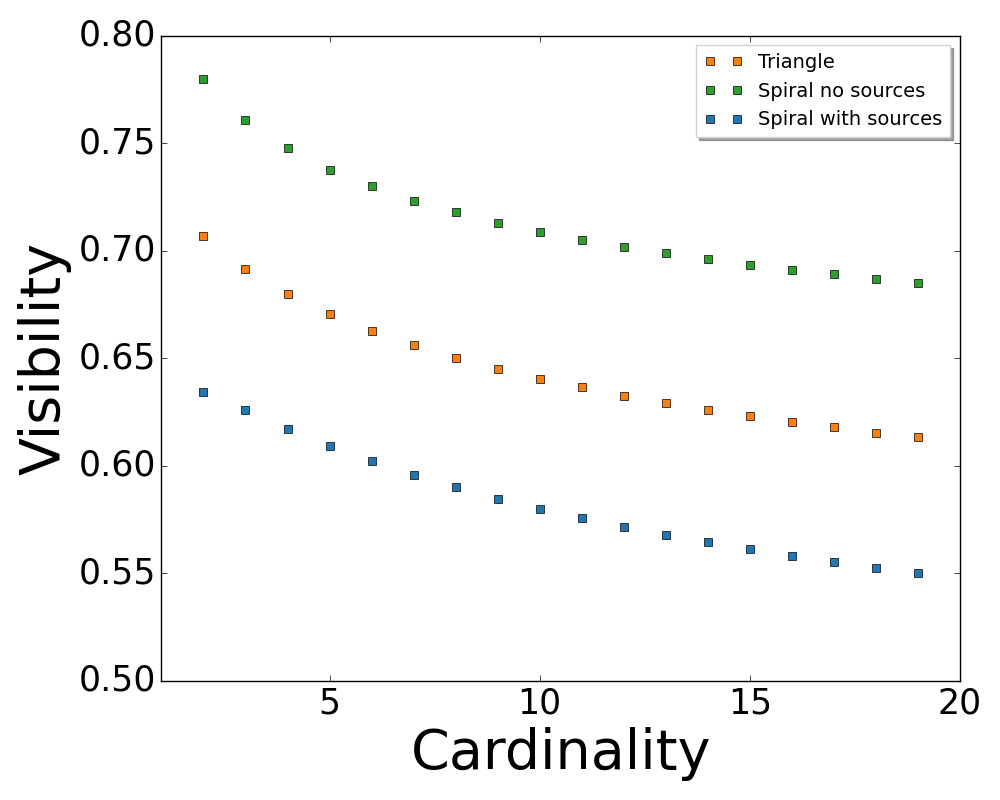
\includegraphics[width=0.5\linewidth]{visibility.png}
    \caption{GHZ visibility as a function of cardinality $d$.}
    \label{fig:visibility}
\end{figure}
\end{document}